\subsubsection{Interrupts from the Pushbutton KEY Port}

Figure \ref{fig:pushbutton_port}, reproduced as Figure \ref{fig:pushbutton_port_int},
shows the registers associated with the pushbutton KEY port. 
The {\it Interruptmask} register allows interrupts to be generated when a key is
pressed. Interrupts can be enabled individually for each key by setting its 
{\it Interruptmask} bit to 1.  When a key is pressed, the corresponding bit in the 
{\it Edgecapture} register is set to 1 by the parallel port. This bit remains 1
until cleared to 0 by software.  An interrupt service routine can read the {\it Edgecapture} 
register to determine which key/s has/have been pressed.  An {\it Edgecapture} register bit can 
be cleared by writing a logic value 1 into the bit position.  Clearing the
bit resets the corresponding interrupt signal being sent to the \GIC.

\begin{figure}[h!]
   \begin{center}
       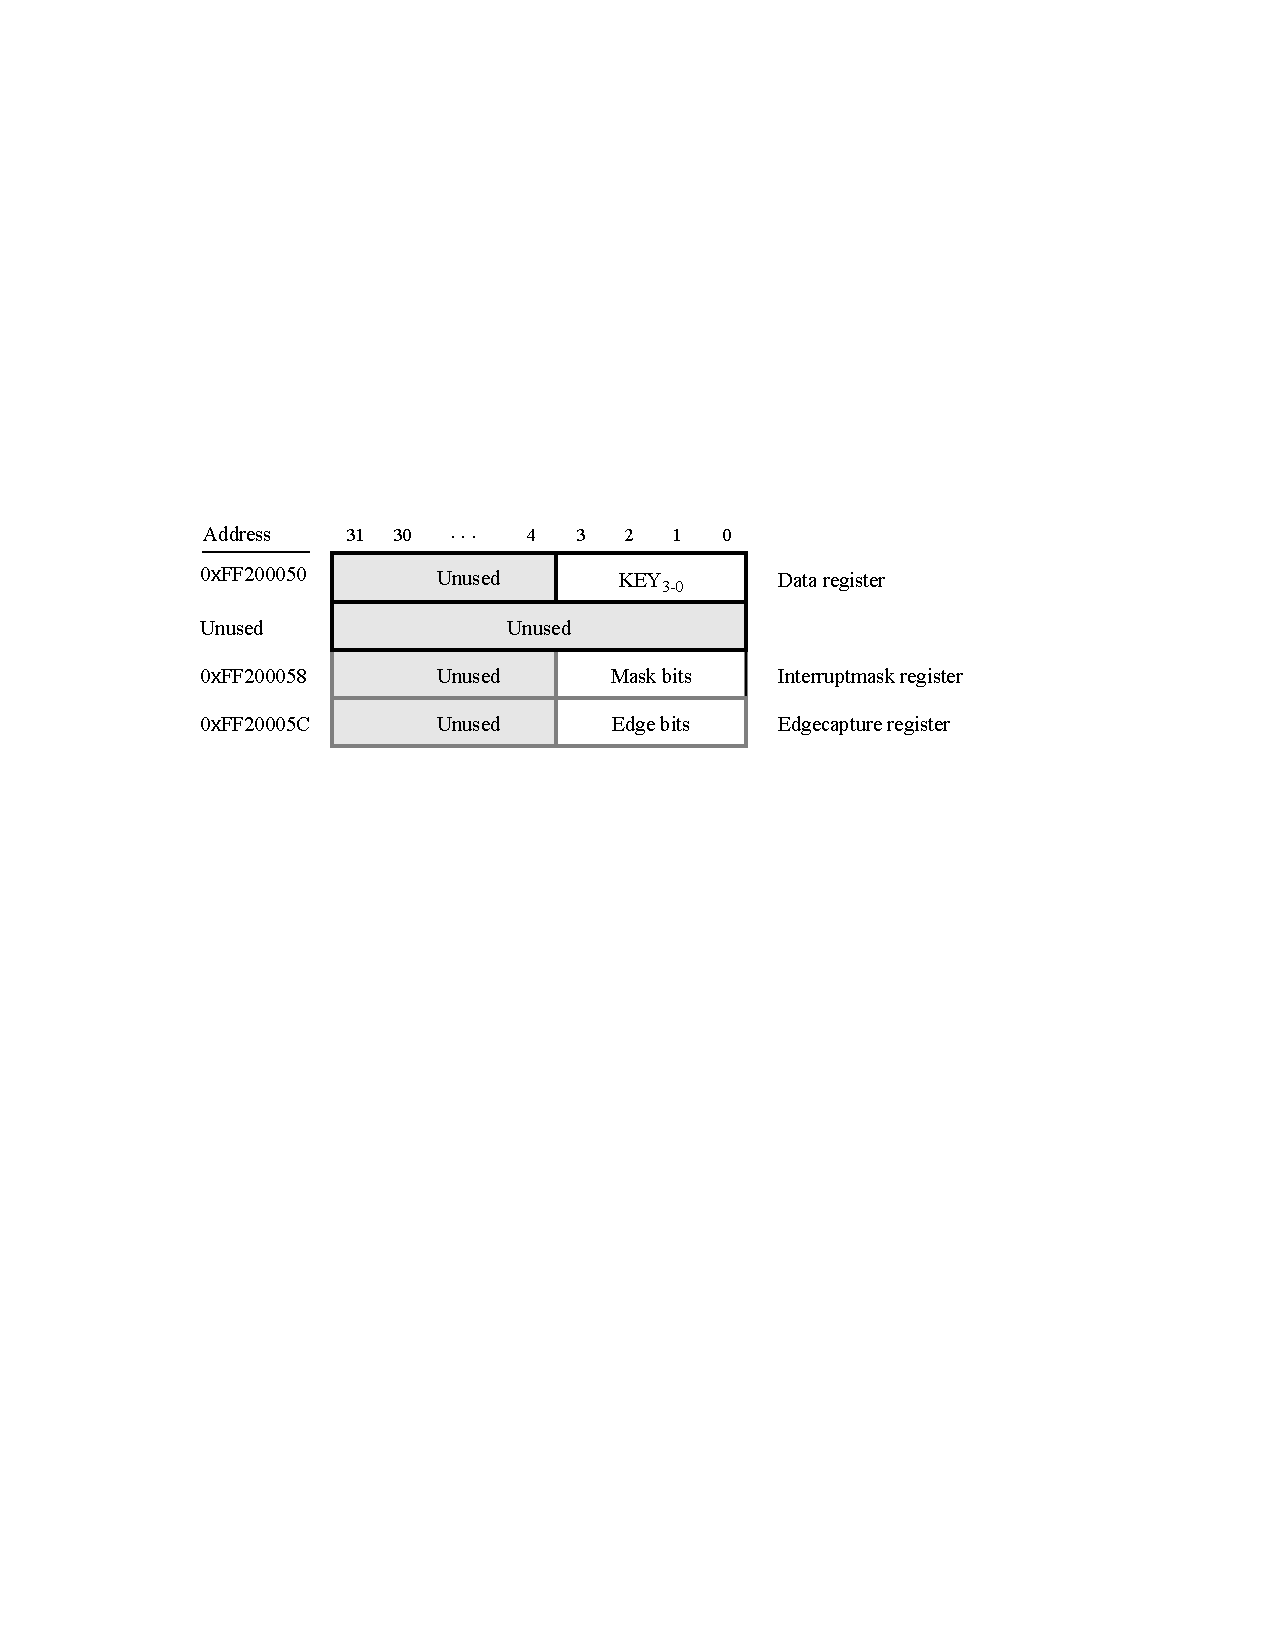
\includegraphics{../../../common/figs/FPGA_PP_Keys.pdf}
   \end{center}
   \caption{Registers used for interrupts from the pushbutton KEY port.}
	\label{fig:pushbutton_port_int}
\end{figure}

